\chapter{วิธีการทดลอง}
\label{chapter:experiment}


% Set Function Names
\SetKwFunction{FMain}{Main}
\SetKwFunction{FLogin}{Login}
\SetKwFunction{FUrl}{GetUrl}
\SetKwFunction{FData}{getData}

ในบทนี้จะกล่าวถึงขั้นตอนและกรอบการทำงานในการพัฒนาระบบแนะนำตำแหน่งงาน การจัดการข้อมูล และการพัฒนาเว็บแอพพลิเคชั่น โดยมีจุดประสงค์เพื่อทำให้ระบบแนะนำตำแหน่งงานสามารถทำงานได้อย่างมีประสิทธิภาพสามารถใช้งานได้จริง รวมถึงอภิปรายภาพรวมระบบทั้งหมด



\section{สถาปัตยกรรมสำหรับไปป์ไลน์ข้อมูล}
สถาปัตยกรรมที่ผู้เขียนเลือกใช้นั้นเป็นเทคโนโลยีโอเพนซอร์สทั้งหมดเพื่อทำให้ทุกขั้นตอนของท่อส่งข้อมูลสามารถทำงานจริงได้ในระยะยาวโดยคำนึงถึงต้นทุนและประสิทธิภาพที่ตามมา
\subsection{โครงสร้างพื้นฐานของระบบ} 
บนเครื่องเซิร์ฟเวอร์นั้นทางผู้เขียนได้เลือกเทคโนโลยี docker เข้ามาใช้ในการจำลองเครื่องเสมือนโดยแบ่งบริการเป็นคอนเทนเนอร์ต่าง ๆ 
เพื่อความง่ายในการควบคุมและจัดการตัวบริการนั้น ๆ อีกทั้งสามารถสเกลได้เมื่อบริการนั้นมีการใช้งานในปริมาณที่มากในอนาคตและง่ายต่อการติดตั้งเมื่อมีการย้ายเซิร์ฟเวอร์
โดยบริการที่ทำงานอยู่บน docker เช่น ฐานข้อมูล ระบบจัดการตารางาน ระบบสกัดข้อมูล โมดูลทำความสะอาดและแปลงข้อมูล โมดูลจำแนกประเภทกลุ่มของข้อมูล ระบบแนะนำ บริการเว็บเซอร์วิส เป็นต้น
\newline

\begin{figure}[!h]
  \centering
  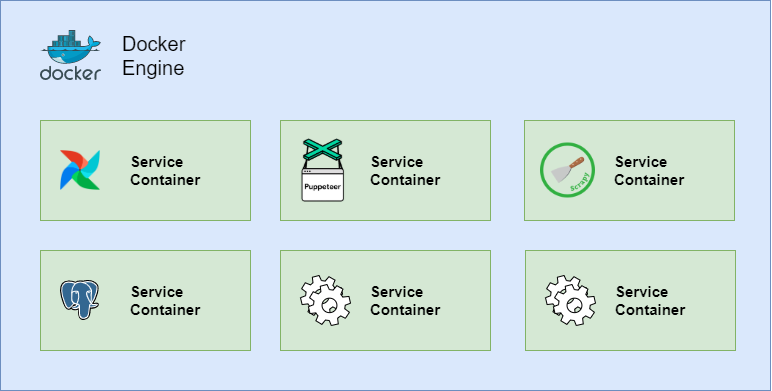
\includegraphics[width=0.8\textwidth]{structure_docker.png}  
  \caption{รูปภาพกรอบการทำงาน บริการที่ทำงานอยู่บน docker engine}
  \label{Fig:data-collection}
\end{figure}

\subsection{แพลตฟอร์มจัดการเวิร์กโฟลว์}
Apache airflow เป็นแพลตฟอร์มการจัดการเวิร์กโฟลว์สามารถกำหนดเวลาหรือขั้นตอนการทำงานได้ด้วยการเขียนโปรแกรมผ่าน python โดยแพลตฟอร์มนี้ถูกต้องตั้งเป็นบริการอยู่บน docker engine 
เพื่อทำการควบคุมตารางการทำงานและโฟลว์ของเคนเทนเนอร์อื่น ๆ โดยมีลำดับการทำงานดังนี้


\subsection{การรวบรวมข้อมูล}
การรวบรวมข้อมูลมีการรวบรวมจากสองแหล่งคือเว็บไซต์ linkedin และเว็บไซต์ indeed โดยทั้งสองเว็บไซต์นี้มีขั้นตอนการสกัดและรวบรวมไม่เหมือนกันโดยเว็บไซต์ linkedin มีความซับซ้อนและความยากในการสกัดข้อมูลมากเนื่องจากเป็นเว็บไซต์ระดับโลกที่มีการป้องกันบอทและการเข้าถึงต่าง ๆ ที่ไม่ใช่มนุษย์อีกทั้งหน้าเว็บยังมีการทำงานเป็นแบบ client-side rendering ซึ่งจำเป็นต้องใช้การจำลองเสมือนมนุษย์มาทำหน้าที่เป็นบอทผ่านไลบรารี่ puppeteer ส่วนเว็บไซต์ indeed เนื่องจากมีการทำงานเป็น server-side rendering จึงสามารถดึงข้อมูลได้ตรงจากการสร้างคำร้องไปที่เซิฟเวอร์และเซิฟเวอร์จะตอบกลับมาเป็นหน้าเว็บเพจที่เป็น static
\newline
\begin{figure}[!h]
  \centering
  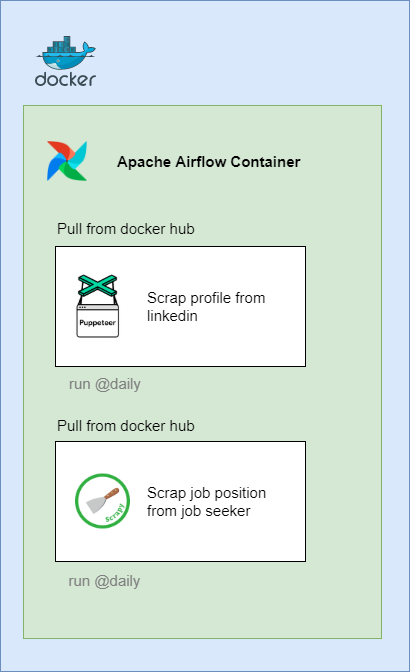
\includegraphics[height=0.7\textwidth]{structure_airflow.png}  
  \caption{รูปภาพกรอบการทำงาน การรวบรวมข้อมูลภายใต้ Airflow}
  \label{Fig:data-collection}
\end{figure}
ทั้งนี้การสกัดข้อมูลจำเป็นต้องมีคำสำคัญหรือเป้าหมายที่เจาะจงในการสกัดข้อมูล ทางผู้จัดทำได้รวบรวมตำแหน่งงานทางเทคโนโลยีสารสนเทศโดยอิงจาก CompTIA certification roadmap โดยแบ่งสายงานทางเทคโนโลยีสารสนเทศเป็นทั้งหมด 8 สายงานและ 62 ตำแหน่งดังนี้
\newpage

\begin{enumerate}
  \item \textbf{service and infrastructure}
  \newline
  helpdesk,
  system admin, 
  virtualization engineer, 
  system engineer, 
  system architect
    
  \item \textbf{network technology}
  \newline
  network technician, 
  network analyst, 
  telecommunication, 
  network security, 
  network admin, 
  network engineer

  \item \textbf{it business and strategy}
  \newline
  it operation, 
  business architect, 
  business analyst, 
  policy advisor, 
  policy consultant, 
  enterprise architect

  \item \textbf{it management}
  \newline
  it manager, 
  it deputy director, 
  it director, 
  project manager, 
  program manager, 
  cto, 
  cio

  \item \textbf{information security}
  \newline
  security trainee, 
  security technician, 
  security analyst, 
  security manager, 
  security engineer, 
  security architect, 
  it auditor, 
  risk compliance, 
  incident, 
  forensics, 
  malware developer

  \item \textbf{devops and cloud technology}
  \newline
  sysops engineer, 
  devops admin, 
  devops engineer, 
  reliability engineer, 
  devops consultant, 
  cloud engineer, 
  cloud architect

  \item \textbf{storange and data}
  \newline
  data center, 
  data analyst, 
  database admin, 
  business intelligence, 
  data warehouse, 
  data scientist, 
  database architect, 
  data engineer, 
  database engineer

  \item \textbf{software development}
  \newline
  software developer, 
  software tester, 
  software support, 
  applications developer, 
  qa, 
  web developer, 
  applications security, 
  web manager, 
  software engineer, 
  software architect, 
  software system architect
\end{enumerate}

\begin{figure}[!h]
  \centering
  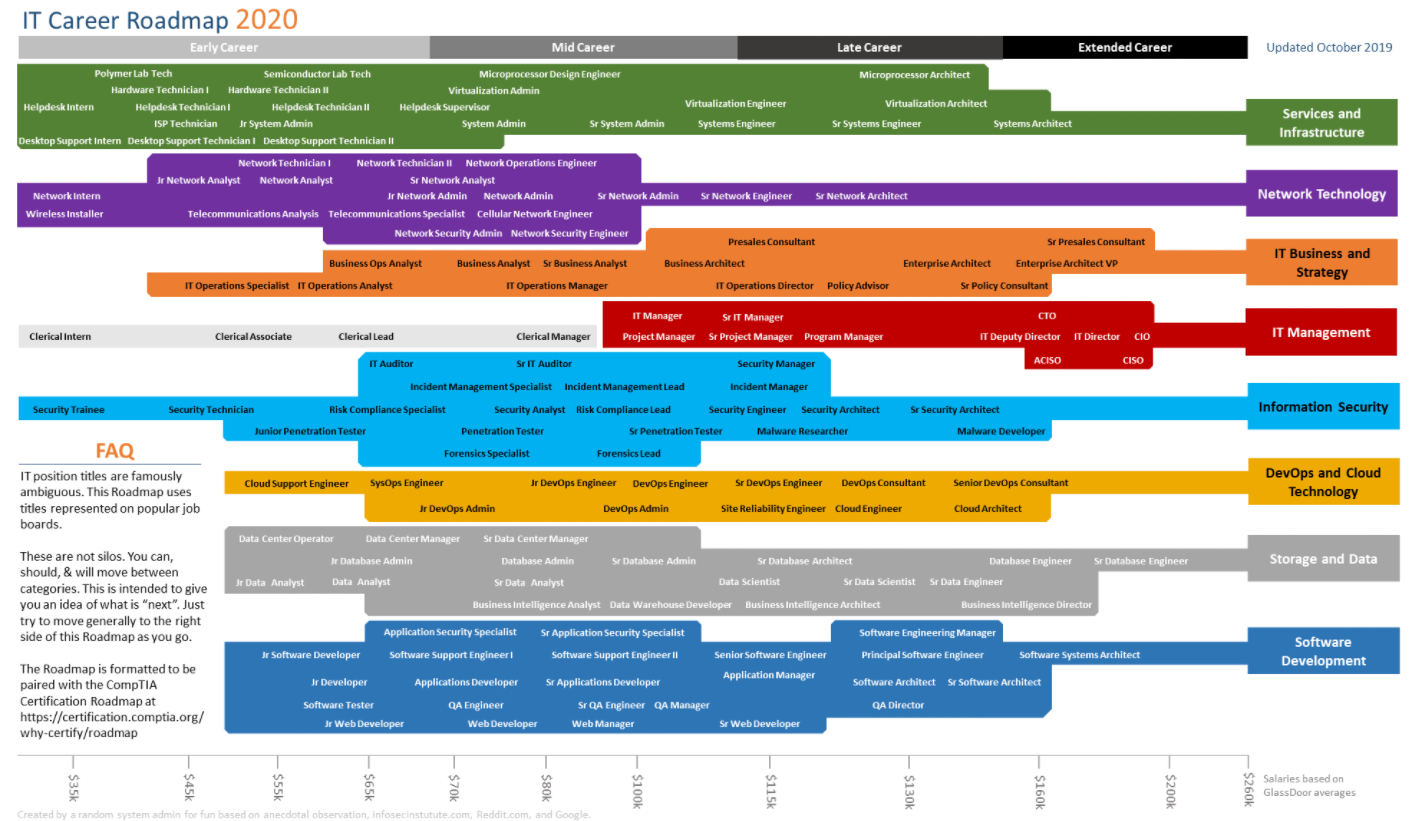
\includegraphics[width=1\textwidth]{chapter3/it_roadmap.png}  
  \caption{it roadmap}
  \label{Fig:it-roadmap}
\end{figure}
\newpage

\subsubsection{Linkedin}
การสกัดข้อมูลโปรไฟล์ผู้ใช้งานลิงค์อินจะใช้ไลบรารี่ puppeteer มาใช้ในการจำลองการกระทำของมนุษย์โดยมีกระบวนการหลักทั้งหมดสามขั้นตอนคือ
\begin{enumerate}
  \item การกำหนดรายการคำสั่งสำหรับการสกัดข้อมูล
  \begin{figure}[!h]
    \centering
    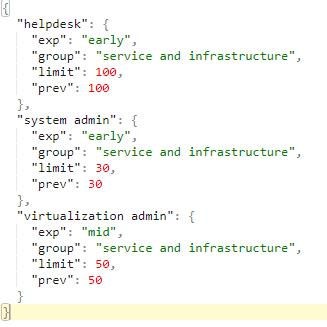
\includegraphics[width=0.4\textwidth]{chapter3/order.jpg}  
    \caption{ไฟล์รายการคำสั่งสกัดข้อมูลบางส่วน}
    \label{Fig:scrap-order}
  \end{figure}
  \item สกัดยูอาร์แอลโปรไฟล์ผู้ใช้จากการค้นหาผ่านคำสำคัญที่กำหนดในรายการคำสั่ง
  \item สกัดข้อมูลโปรไฟล์ผู้ใช้จากการเข้าสู่หน้าหลักโปรไฟล์ผ่านยูอาร์แอลที่สกัดมาจากขั้นตอนก่อนหน้า
\end{enumerate}

\begin{algorithm}
\DontPrintSemicolon
  \SetKwProg{Fn}{Function}{:}{}
  \Fn{\FMain{$order$}}{
    Login(env.username, env.password)\;
    GetUrl()\;
    GetData()\;
  }

  \SetKwProg{Fn}{Function}{:}{}
  \Fn{\FLogin{$username$, $password$}}{
    \eIf{exist cookies}{
      login with cookie\;
    }{
      login with username, password form\;
    }
    save cookie\;
  }

  \SetKwProg{Fn}{Function}{:}{}
  \Fn{\FUrl{}}{
    read order\;
    read backlist\;
    \If{not exist backlist}{
      generate backlist file from order\;
    }
    \While{order}{
      profiles = []\;
      \While{order.keyword}{
        search keyword\;
        scroll all page\;

        urls = querySelectorAll(all profile).href\;
        urls = backlist filter(urls)\;
        urls = realurl filter(urls)\;

        profiles.push(url)\;
      }
      save profiles to file\;
      update order file\;
      update backlist file\;
    }
  }

  \SetKwProg{Fn}{Function}{:}{}
  \Fn{\FData{}}{
    read url files
    \While{files}{
      data = []\;
      \While{files.url}{
        goto url\;
        validate page is exist\;
        scroll all page\;
        scrap name\;
        scrap about\;
        scrap experience\;
        scrap skill\;
        scrap interest\;

        data.push({name, about, experience, skill, interest})\;
      }
      save data to file\;
    }
  }

  \caption{Scrap profile algorithms}
\end{algorithm}

\subsubsection{Indeed}
การสกัดข้อมูลตำแหน่งงานจากเว็บไซต์อินดีดจะใช้เฟรมเวิร์ค scrapy มาใช้ในการรวบรวมข้อมูลจากรีเครสที่ส่งไปเพื่อค้นหาตำแหน่งงานจากคำสำคัญที่กำหนดไว้ โดยจะมีขั้นตอนการทำงานหลักสามขั้นตอนคือ
\begin{enumerate}
  \item การกำหนดรายการคำสั่งสำหรับการสกัดข้อมูล
  \begin{figure}[!h]
    \centering
    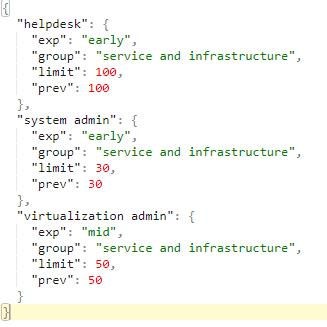
\includegraphics[width=0.4\textwidth]{chapter3/order.jpg}  
    \caption{ไฟล์รายการคำสั่งสกัดข้อมูลบางส่วน}
    \label{Fig:scrap-order}
  \end{figure}
  \item สกัดยูอาร์แอลตำแหน่งงานจากการค้นหาผ่านคำสำคัญที่กำหนดในรายการคำสั่ง
  \item สกัดข้อมูลหน้าตำแหน่งงานจากการเข้าสู่หน้าตำแหน่งงานจากยูอาร์แอลที่สกัดมาจากขั้นตอนก่อนหน้า
\end{enumerate}


\subsection{การจัดการข้อมูล}
หลังจากทำการรวบรวมข้อมูลจากทั้งสองแหล่ง (linkedin, indeeed) และบันทึกเป็นรูปแบบไฟล์อยู่ในทะเลสาบข้อมูลแล้ว airflow จะทำการรันและเริ่มกระบวนการทำความสะอาดข้อมูล(Data cleansing) โดยเป็นกระบวนการตรวจสอบแก้ไขหรือลบรายการข้อมูลที่ไม่ถูกต้องหรือไม่สอดคล้องออกจากชุดข้อมูลโดยมีขั้นตอนดังนี้
\begin{enumerate}
  \item ตรวจสอบฟอร์แมทและความถูกต้องของไฟล์ข้อมูล
  \item ลดรูปข้อมูลที่ซ้ำกัน ถ้าข้อมูลระบุกลุ่มที่แตกต่างกันให้รวมกลุ่มนั้นเป็นหลายรายการในข้อมูลเดียว
  \item ลบข้อมูลที่ไม่มีฟีเจอร์สำคัญคือฟีเจอร์ about และ skill
  \item ข้อมูลที่ผ่านขั้นตอนทั้งหมดจะถูกบันทึกลงฐานข้อมูลโดยมีรูปแบบที่ชัดเจนและพร้อมใช้งาน
\end{enumerate}

\begin{figure}[!h]
  \centering
  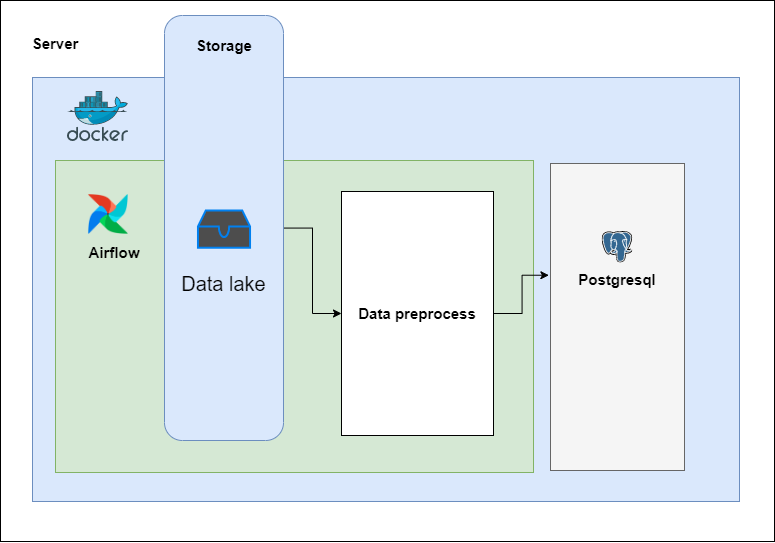
\includegraphics[width=0.8\textwidth]{structure_preprocess.png}  
  \caption{รูปภาพโฟลว์การทำงานของการจัดการข้อมูล}
  \label{Fig:data-collection}
\end{figure}



\subsection{การเทรนโมเดลแบ่งกลุ่มสายงาน}
  ในการเทรนโมเดลมีขั้นตอนหลายอย่างที่ต้องคำนึงถึง เพื่อให้โมเดลมีความแม่นยำในการแบ่งสายงาน จึงจำเป็นต้องนำเทคนิคต่าง ๆ มาประยุกต์ใช้ทั้งกับในด้านข้อมูลและด้านโมเดล โดยเทคนิคหลักที่นำมาใช้มีดังนี้
  \subsubsection*{การทำความสะอาดข้อมูล}
    ก่อนขั้นตอนการเทรนโมเดล ข้อมูลจำเป็นต้องอยู่ในรูปแบบที่เหมาะสมต่อการใช้ในการเทรนโมเดลมากที่สุดโดยขั้นตอนการ "clean data" จะประกอบไปด้วยขั้นตอนง่ายๆ ทั่วไปอย่างเช่น 
    \begin{enumerate}
      \item การเปลี่ยนข้อมูลให้เป็นตัวเล็ก อักขระพิเศษทั้งหมด ลบตัวอักษรโดด ลบแท็ก ลบช่องว่างที่เกินกำหนด
      \item การใช้ "stopword" คัดกรองคำที่ไม่จำเป็นออกจากข้อมูล
      \item ใช้เทคนิค"Lemmatizer" หรือการลดรูปคำให้เป็นคำรากศัพท์เช่น "am", "are", "is" จะถูกเปลี่ยนเป็น "be" 
      \item ใช้เทคนิค "Tokenize" หรือเทคนิคการแบ่งคำมาแบ่งข้อมูลให้อยู่ในรูปแบบโทเค็นหรือในรูปแบบคำต่อคำ
      \item พิจารณ์รูปแบบของคำที่สะกดผิดเช่น "cool", "kewl", "cooool"
    \end{enumerate}
    
  \subsubsection*{การสร้างโครงสร้างของคำ}
  เมื่อทำความสะอาดข้อมูลแล้วจะสังเกตุว่าข้อมูลยังมีการกระจายที่ยังไม่แน่นอนและไม่สามารถแยกแยะด้วยตาเปล่าได้ เทคนิคต่อไปนี้เป็นการทำให้ข้อมูลมีความชัดเจนมากยิ่งขึ้นโดยมีขั้นตอนดังนี้
  \begin{figure}[!h]
    \centering
    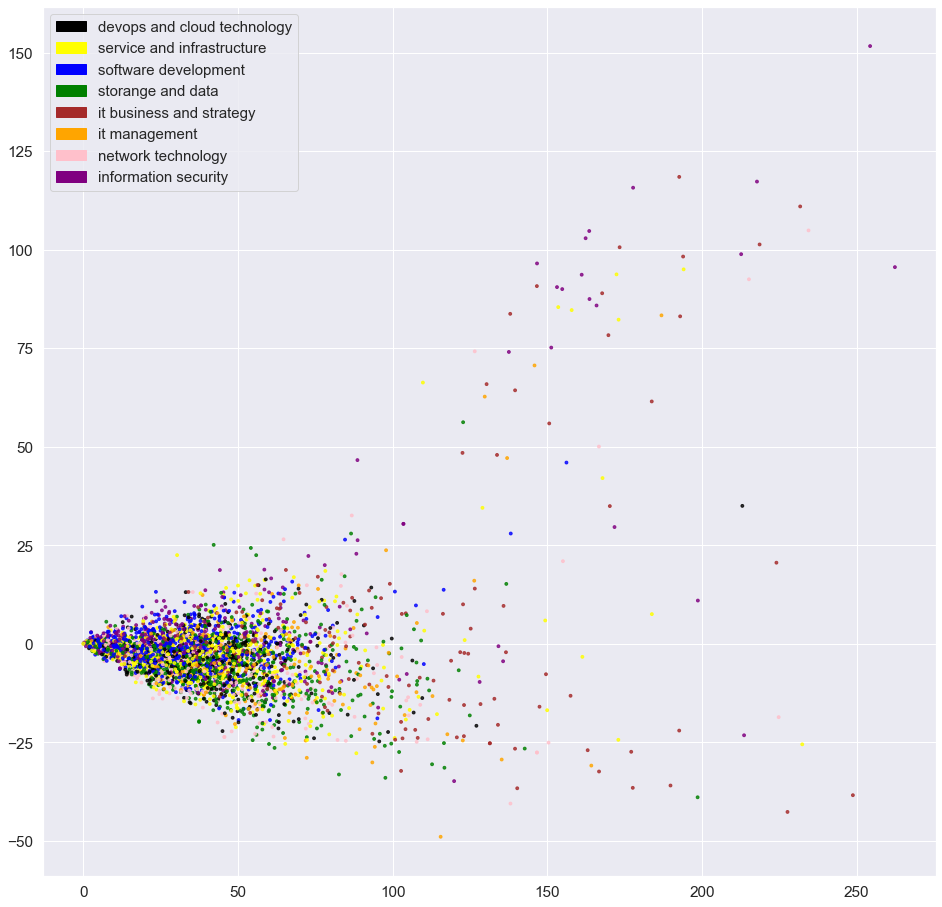
\includegraphics[width=1\textwidth]{chapter3/pca_counts.png}  
    \caption{PCA vector ของตำแหน่งงานเมื่อทำความสะอาดข้อมูลแล้ว}
    \label{Fig:pca-count}
  \end{figure}

  \paragraph*{TF-IDF} เพื่อช่วยให้โมเดลสามารถโฟกัสความหมายของคำได้จึงได้นำเทคนิค "TF-IDF (Term Frequency, Inverse Document Frequency)" เข้ามาใช้ในการให้น้ำหนักคำตามความหายากในชุดข้อมูล และลดคำที่เกิดขึ้นบ่อยเกินไปแล้วไปเพิ่ม noise ให้กับข้อมูลโดยรวม \par
  \begin{figure}[!h]
    \centering
    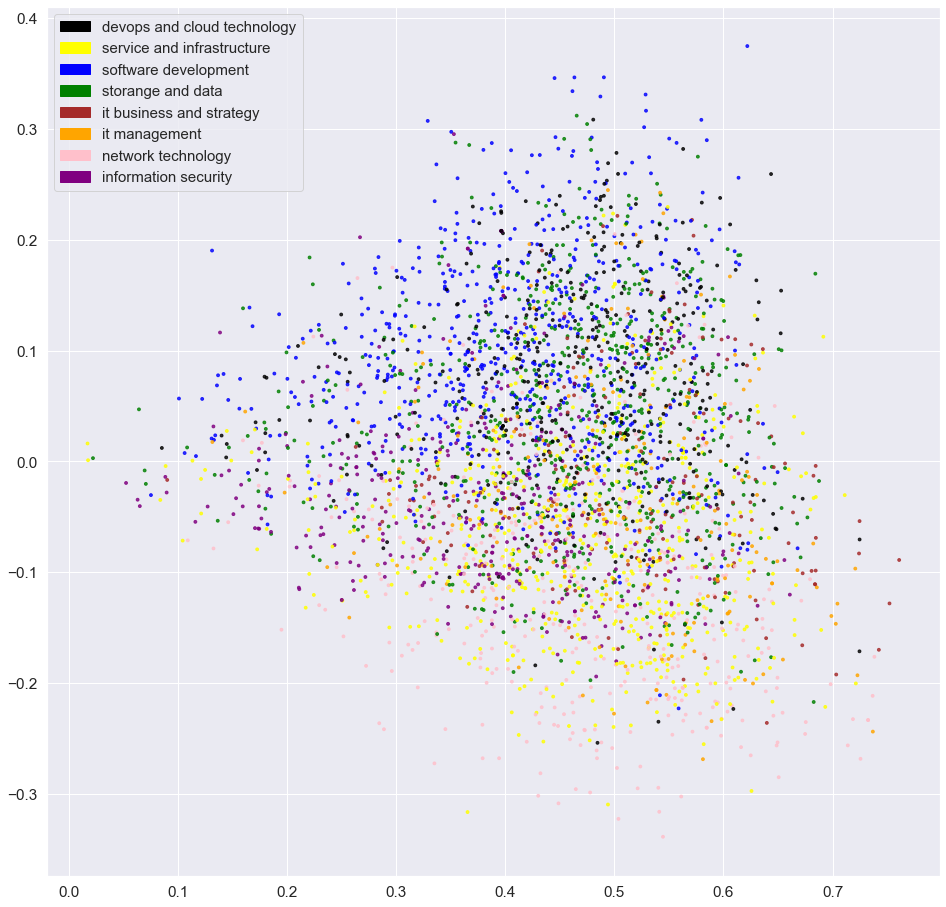
\includegraphics[width=1\textwidth]{chapter3/pca_tfidf.png}  
    \caption{PCA vector ของตำแหน่งงานเมื่อทำการให้น้ำหนักแก่คำแล้ว}
    \label{Fig:pca-tfidf}
  \end{figure}

  \paragraph*{Word2Vec} ถึงจะสามารถจัดการกับความถี่ของคำได้แล้ว แต่อย่างไรก็ตามมีความเป็นไปได้มากว่า หากเราปรับใช้โมเดลนี้เราจะพบคำศัพท์ที่เราไม่เคยเห็นในชุดข้อมูลของเรามาก่อน รุ่นก่อนหน้านี้อาจไม่สามารถจำแนกคำเหล่านี้ได้อย่างถูกต้องแม้ว่าคำจะเป็นคำที่คล้ายกันมากในการเทรนก็ตาม เพื่อแก้ปัญหานี้ การจับความหมายของคำ "semantic meaning of word" โดยเครื่องมือที่ใช้เพื่อจับความหมายเรียกว่า "Word2Vec" \par
    \subparagraph{pre-trained words} word2vec เป็นเทคนิคในการการฝังคำอย่างต่อเนื่อง(continuous embeddings) โดยเรียนรู้จักการอ่านข้อความจำนวนมากและจดจำคำที่มีแนวโน้มที่ปากฎในบริบทที่คล้ายคลึงกัน หลังจากที่เทรนมามากพอแล้วจะสร้างเวกเตอร์ 300 มิติ สำหรับแต่คำแต่ละคำในคำศัพท์ โดยคำที่มีความหมายใกล้เคียงกันจะมีระยะใกล้เคียงกัน
    โดยผู้จัดทำได้นำ pre-trained ของ "GoogleNews" ที่ประกอบไปด้วยเวกเตอร์ของคำมากกว่า 3 ล้าน หลังจากการทำ word embeddings ด้วย word2vec แล้วจะสังเกตุว่าการกระจายตัวมีความแน่นหนาขึ้นแต่การแบ่งแยกสายงานไม่แตกต่างจากการทำ TFIDF มากนัก
    \begin{figure}[!h]
      \centering
      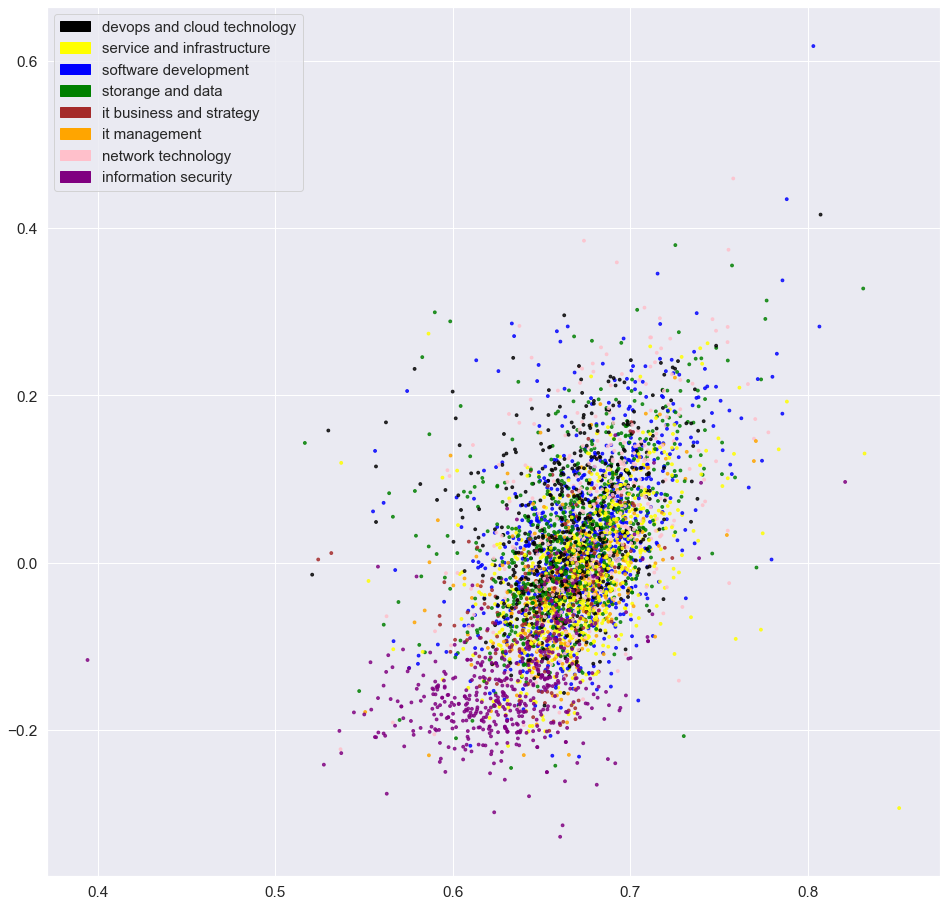
\includegraphics[width=0.8\textwidth]{chapter3/pca_word2vec.png}  
      \caption{PCA vector ของตำแหน่งงานผ่านเทคนิค word2vec}
      \label{Fig:pca-tfidf}
    \end{figure}
  
  \newpage
  หลังจากที่ข้อมูลอยู่ในรูปแบบที่พร้อมใช้งานแล้วจึงนำข้อมูลมาทำการสร้างโมเดลแบ่งกลุ่มตำแหน่งงาน โดยกลุ่มจะถูกแบ่งออกเป็นทั้งหมด 8 กลุ่มใหญ่และ 62 ตำแหน่งงาน \cite[CompTIA]{comptia} โดยมีลักษณะดังนี้\newline

  \begin{figure}[!h]
    \centering
    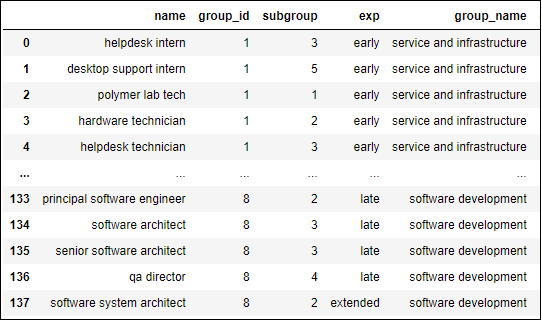
\includegraphics[width=0.7\textwidth]{structure_comptia.png}  
    \caption{กลุ่มงานทางไอที}
    \label{Fig:structure_comptia}
  \end{figure}

  การเทรนโมเดลนั้นจะถึงสั่งการโดย airflow ให้ทำการเทรนทุก ๆ หนึ่งวันเพื่อเป็นการอัพเดทตัวโมเดลให้มีความแม่นยำและถูกต้องมากที่สุดและโมเดลที่ทำการเทรนจะถูกเก็บไว้ที่ storage ของเซิร์ฟเวอร์รอถูกเรียกใช้โดยระบบแนะนำต่อไปโดย ทั้งนี้ตัวโมเดลจะใช้เทคนิค "support vector machine" เข้ามาใช้ในการเทรนโมเดลโดยตัวอย่างไปป์ไลน์ที่ใช้ในการเทรนมีเดลจะมีลักษณะดังนี้
  \begin{figure}[!h]
    \centering
    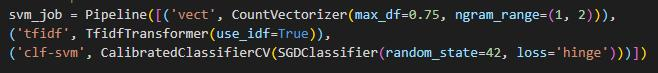
\includegraphics[width=1\textwidth]{chapter3/svm_pipline.jpg}  
    \caption{ตัวอย่างโค้ดไปป์ไลน์เทรนโมเดล}
    \label{Fig:svm_pipline}
  \end{figure}


\subsection{ระบบแนะนำ}

ระบบแนะนำ จะใช้เทคนิคการกรองโดยอิงจากเนื้อหาโดยเบสข้อมูลที่แตกต่างกันคือ ข้อมูลยูสเซอร์เบส และข้อมูลจ็อบเบส โดยการเลือกกลุ่มงานจะอ้างอิงจากระยะทางของยูสเซอร์และจ็อบด้วยระยะทางโคไซน์ (cosine distance) โดยการนำโมเดล SVM ที่เทรนจากข้อมูลที่แตกต่างกันมาเข้ามาใช้ในการทำนาย
\begin{algorithm}
  \DontPrintSemicolon
  \SetKwProg{Fn}{Function}{:}{}
  \Fn{Main(payload): Response(Record<string, any>[])}{
    read jobs from db\;
    read profiles from db\;
    load job-based pre-train model\;
    load profile-based pre-train model\;
    load accuracy weight by model

    return recommendation([job model, profile model], payload, jobs, acc, 20)
  }

  \SetKwProg{Fn}{Function}{:}{}
  \Fn{recommendation(models, payload, jobs, acc, n): Record<string, any>[]}{
    
    payload = clean payload text\;
    groups = predict `payload` in each `models'\;
    jobs = filter all jobs by groups(labels)\;
    acc = calculate accuracy in each group by weight 100\% \;
    jobs\_sim = calculate similarity between all job and payload then drop duplicate\;
    result = sort similarity job jobs\_sim \;
    return result[:n]\;
  }

  \caption{Job recommendation algorithm}
\end{algorithm}

\begin{figure}[!h]
  \centering
  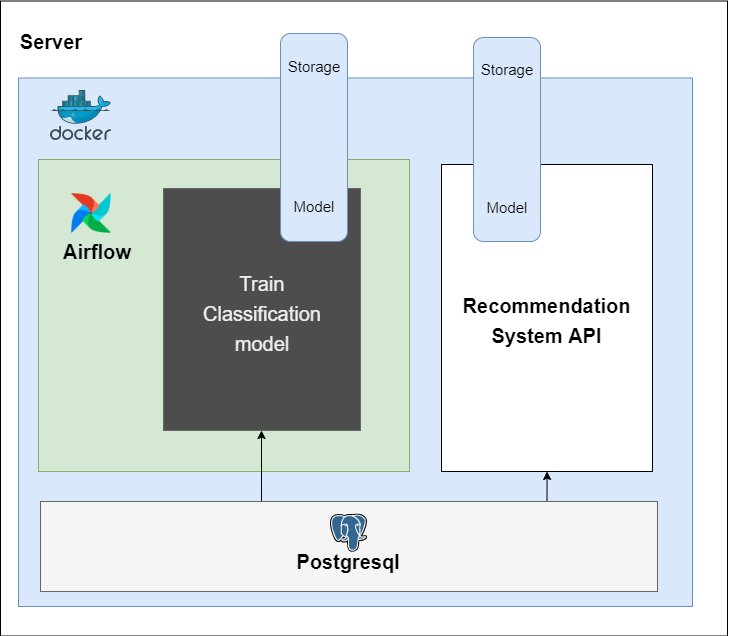
\includegraphics[width=0.7\textwidth]{structure_recomm.png}  
  \caption{รูปภาพโฟลว์การทำงานระบบแนะนำ}
  \label{Fig:strucutre_recomm}
\end{figure}


\pagebreak

\section{การพัฒนา API เพื่อให้บริการระบบแนะนำ}
ในการพัฒนา API เพื่อให้บริการระบบแนะนำนั้นผู้จัดทำได้เลือกเฟรมเวิร์คที่มีความคุ้นชินและเหมาะสมในการพัฒนามากที่สุดโดยเฟรมเวิร์คที่เลือกนั้นคือเฟรมเวิร์คของภาษา "python" ที่ชื่อว่า "flask" มาพัฒนาเป็น API โดยมีขั้นตอนดังนี้
\begin{enumerate}
  \itemsep0em 
  \item ออกแบบผังระบบ (Context Diagram)
  \item ผังการแยกฟังก์ชั่นงานย่อย (Decomposition Diagram)
  \item ออกแบบฐานข้อมูลเชิงคุณภาพ (Physical Design)
\end{enumerate}
\newpage

\subsection{ออกแบบผังระบบ (Context Diagram)}
  \begin{figure}[!h]
    \centering
    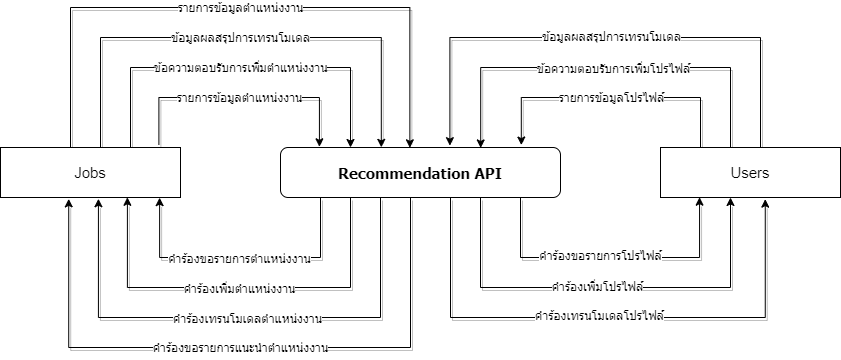
\includegraphics[width=1\textwidth]{chapter3/context-diagram.png}  
    \caption{context diagram}
    \label{Fig:context_diagram}
  \end{figure}

\subsection{ผังการแยกฟังก์ชั่นงานย่อย (Decomposition Diagram)}
  \begin{figure}[!h]
    \centering
    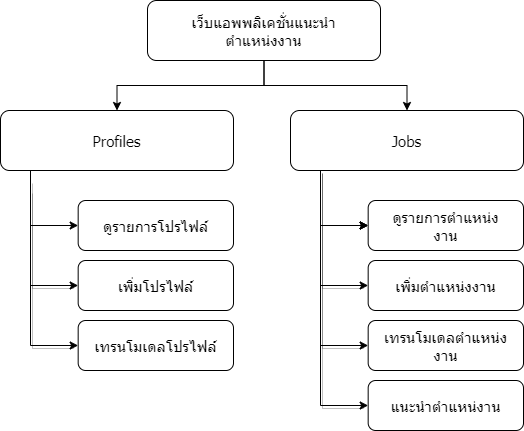
\includegraphics[width=0.8\textwidth]{chapter3/decomposiiton-diagram.png}  
    \caption{decomposiiton diagram}
    \label{Fig:decomposiiton_diagram}
  \end{figure}
  \newpage

\subsection{ออกแบบฐานข้อมูลเชิงคุณภาพ (Physical Design)}
\begin{figure}[!h]
  \centering
  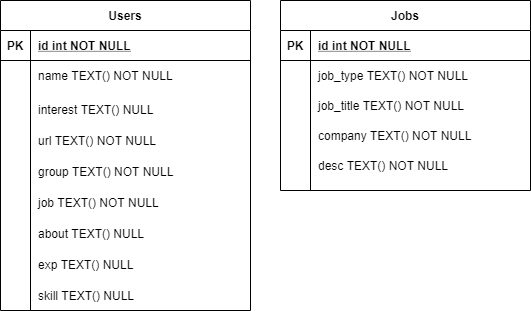
\includegraphics[width=0.8\textwidth]{chapter3/physical-diagram.png}  
  \caption{physical diagram}
  \label{Fig:physical_diagram}
\end{figure}



% \begin{figure}[!h]
%   \centering
%   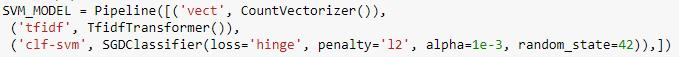
\includegraphics[width=0.95\textwidth]{model_pipeline.jpg}  
%   \caption{การสร้างขั้นตอนโมเดลด้วยไปป์ไลน์}
%   \label{Fig:data-prepare}
%   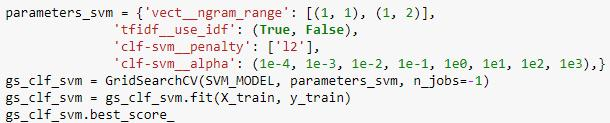
\includegraphics[width=0.95\textwidth]{model_optimize.jpg}  
%   \caption{การเลือกตัวแปรที่ดีที่สุดให้แก่โมเดล}
%   \label{Fig:data-prepare}
% \end{figure}



